\chapter{Literaturjiddisch als Sprachzeugnis des Westjiddischen}\label{sekundaerquelle}
% \epigraph{\textit{Se non è vero, è ben trovato.}}{--- \textup{Giordano Bruno \\ (\qu{De gli eroici furori} 2.3)}} %Seconda parte. Dialogo terzo %LS! in text einbinden?
    
  %  %\noindent
Die gewonnenen Analyseergebnisse der zwei Korpora des Literaturjiddischen erlauben nun die in Abschnitt \ref{lijisprachwissenschaft} (S.\, \pageref{lijisprachwissenschaft}) geäußerten Fragen und Hypothesen zu konkretisieren bzw. zu beantworten. Dies ist die Aufgabe der folgenden zwei Kapitel.

 
Das erstaunlichste Ergebnis der Untersuchung ist, dass sich alle der herausgefilterten Phänomene auf eine tatsächlich westjiddische, ostjiddische oder zumindest deutsch-dialektale Form zurückführen lassen. Dass insgesamt über 60 Einzelphänomene extrahiert werden konnten, spricht nicht nur für die große Flexibilität kontinentalwestgermanischer Sprachen, sondern vor allem für die Authentizitätsanspruch der Imitationen. Tatsächlich ist das Literaturjiddische kein Phantasieprodukt, wie es in den meisten Fällen des Literaturhebräischen der Fall ist (vgl.\, Abschnitt \ref{lihe}, S.\, \pageref{lihe}), sondern die Autoren waren allen Anschein nach um eine Realitätsnähe ihrer Imitationen bemüht. Das Westjiddische hatte als Imitat einen festen Platz in der deutschsprachigen Trivialiteratur des 18. und 19. Jahrhunderts.
 
Das Literaturjiddische ist ein (wenn auch \textit{künstliches}) Resultat des deutsch-jid\-di\-schen Sprach\-kontakts. Die sprachlichen Imitationen können als Perzeptionsdaten genutzt werden oder auch als Sekundärquellen zu den wenigen authentischen westjiddischen Quellen ergänzend herangezogen werden. Hier spielen in Zukunft Daten des Literaturjiddischen vor allem eine Rolle bei der Gewinnung diatopischer  Raumbilder zum Westjiddischen, wo sie als \textit{Lückenfüller} heranzuziehen sind, wie dies exemplarisch am Phänomen der Senkung von /\textit{u}/ > /\textit{o}/ vor <r> in Abbildung \ref{ProtoLCAAJOEWY2} (S.\, \pageref{ProtoLCAAJOEWY2}) gezeigt wurde. Darüber hinaus geben die Phänomene des Literaturjiddischen Hinweise auf interessante Strukturen des West- und auch des Ostjiddischen, die nur sehr niedrigfrequent in authentischen Quellen belegt sind, denen es sich aber lohnt weiter nachzugehen. Weinreichs (\citeyear[62]{Weinreich1953}) Postulat, dass man in Anbetracht der Datenlage zum Westjiddischen diesen problematischen Quelltyp nutzen muss und kann, wurde mit der vorliegenden Untersuchung bestätigt. Daten des \hai{LiJi1} können Lücken zwischen historischen Daten und fehlenden Belegen aus dem späten Westjiddischen füllen, wie z.\,B.\, im Fall der \quein{\textit{kumen} + Bewegungsverb\textsubscript{\textit{zu}-Infinitiv}-Konstruktion} (vgl.\, Kapitel \ref{kommenzugehen}, ab S.\, \pageref{kommenzugehen}) oder der rechtsadjazenten trennbaren Verbpartikeln (vgl.\, Kapitel \ref{rechtsadjazent}, S.\, \pageref{rechtsadjazent}). Letzten Endes muss jedoch jeder literaturjiddische Einzelbeleg geprüft werden und entschieden werden, inwiefern Dialektkompetenz der Autoren oder aber der literarische Diskurs als Störfaktor die \isi{Imitation} des Jiddischen beeinflussen.
 
 \chapter{Strukturen sprachlicher Emulation}\label{lernenimitation}
 
% \epigraph{\textit{In imitating, the person constructs a match between some aspect of the external world and his or her own activity.}}{--- \textup{Ina C.\cite[2]{Uzgiris1981}}}


\noindent Jiddisch ist aufgrund des gemeinsamen mittelhochdeutschen Kerns die dem Deutschen am nächsten verwandte Sprache. Die \isi{Imitation} des Jiddischen durch Sprecher des Deutschen ist besonders durch diese relativ geringe typologische Distanz geprägt. Die Nachahmung einer nahverwandten Varietät  kann, wie im Fall des \hai{{\LiJi}}, als emulierende \isi{Imitation} erfolgen. Dies bedeutet, dass die Grundstruktur der Matrixsprache erhalten bleibt und nur in einzelnen signifikanten Merkmalen manipuliert wird, um die Zielsprache (target language) anzuzeigen. Diese Merkmale können aber auch aus anderen sprachlichen Quellen gespeist werden. Allen voran treten im \hai{{\LiJi}} Reflexe autoreigener Dialektalität auf. Dieser Einfluss ist besonders in Sprachkulturen zu erwarten, in denen eine deutliche Differenz zwischen Dialektalität und Schriftlichkeit gegeben ist. Doch auch Konzepte aus dem indirekten \isi{Sprachkontakt}, wie etwa der literarische Diskus, spielen eine Rolle. Das Ergebnis einer solchen \isi{Emulation} ist eine Überlagerung dieser drei Quellen, die sich im Idealfall aus allen diesen Quellen speist, was an sich aber keine Notwendigkeit darstellt (vgl.\, Abbildung \ref{subtraktiveFarbmischung}). 

% \todo{Die Farben sehen hier blöd aus!}
  \begin{figure}[htbp]
  \farbgrafik %hier kann zur Not auf Farbe verzichtet werden
 \begin{center}
 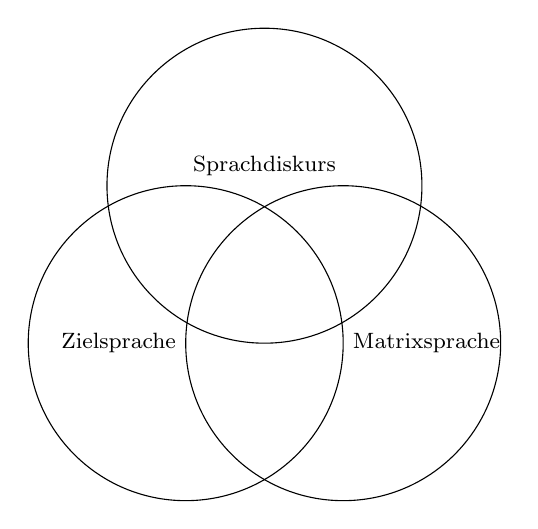
\begin{tikzpicture}
%      \draw [fill=yellow,opacity=0.5] (1.5,2) circle (1) node[above] {\small Sprachdiskurs};
%     \draw [fill=magenta!70,opacity=0.5](1,1) circle (1) node[left] {\small Zielsprache};
%     \draw [fill=cyan!70,opacity=0.5](2,1) circle (1) node[right] {\small Matrixsprache};
     \draw  (3,4) circle (2) node[above] {\footnotesize Sprachdiskurs};
    \draw (2,2) circle (2) node[left] {\footnotesize Zielsprache};
    \draw (4,2) circle (2) node[right] {\footnotesize Matrixsprache};


             \end{tikzpicture}
              \caption{Quellen sprachlicher Imitation}\label{subtraktiveFarbmischung}	
\end{center}
 \end{figure}

 

\noindent Die Möglichkeit zur \textit{Überlagerung} verschiedener sprachlicher Quellen wird als Indiz für die Viskosität der Matrixsprache gedeutet. Diese ermöglicht erst eine Manipulation sprachlicher Strukturen. Wie zugänglich ein sprachliches System für die emulierende \isi{Imitation} ist, wird demnach graduell durch typologische Distanz (Markiertheit vs. Unmarkiertheit) und die Viskosität der Matrixsprache bestimmt (Abbildung \ref{potenzialImitation}). 


\begin{figure}[htbp]
 \begin{center}
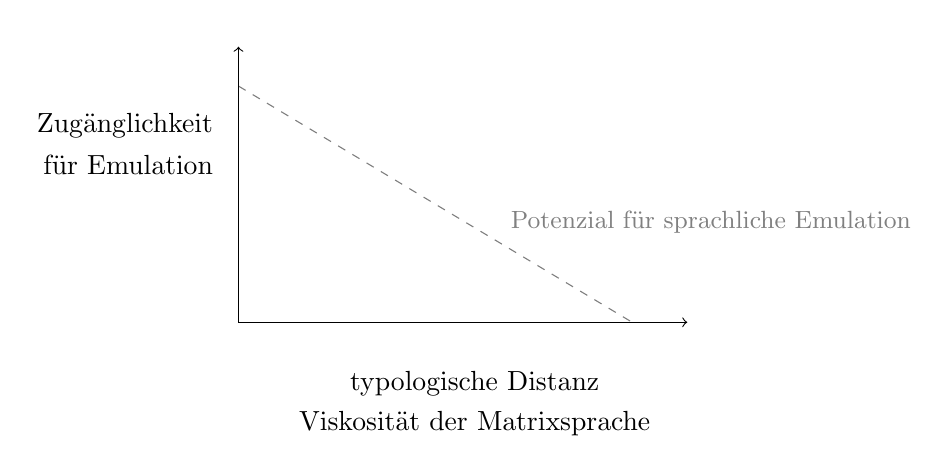
\begin{tikzpicture}
  
% Add dashed line dropping down from normal.
    \draw[dashed, gray] (0,3) -- (5,0);
  \draw[gray] (6,1) node[above] {\small Potenzial für sprachliche Emulation};
  
% Optional: Add axis labels
    \draw (-.2,2.5) node[left] {Zugänglichkeit};
     \draw (-.2,2) node[left] {für Emulation};
    \draw (3,-.5) node[below] {typologische Distanz};
 \draw (3,-1) node[below] {Viskosität der Matrixsprache};
 %\draw (3,-1.5) node[below] {Markiertheit};
 
% Optional: Add axes
    \draw[->] (0,0) -- (5.7,0) node[right] {};
    \draw[->] (0,0) -- (0,3.5) node[above] {};
 
 \end{tikzpicture} \caption{Potenzial für sprachliche Emulation}\label{potenzialImitation}	
\end{center}
 \end{figure}


\noindent Alles in allem finden wir Mechanismen von emulierender \isi{Imitation} auf zwei Ebenen: Zunächst werden sprachliche Konzepte vordergründig wirksam, d.\,h. hier werden einzelne Markierungen zum Zweck der \isi{Emulation} entlehnt. Form, Ausmaß und Überlagerungen dieser Quellen variieren von Autor zu Autor. Hintergrundwirksam sind hingegen typologische Faktoren, die den potenziellen Rahmen sprachlicher \isi{Emulation} festlegen. Die Graphik in Abbildung \ref{beispielpotenzialImitation} illustriert diese Dichotomie vorder- und hintergründiger Wirkmechanismen an einem Beispielsatz. Die Graphik verdeutlicht auch die Problematik der (Re-)Analyse von Imitationsdaten: Auf welche sprachliche Quelle (Diskurs, Zielsprache oder Dialektalität) die \isi{Imitation} letzten Endes aufbaut, ist im Einzelfall oft schwer zu entscheiden. Auch aus diesem Grund sollte im Rahmen weiterer Bearbeitungen des Phänomens der Dialektimitation ein stärkeres Gewicht auf die hintergründig wirksamen Potenziale der Matrixsprache gelegt werden als auf die Interferenzmerkmale. Denn dieser Bereich
liefert im Fall der emulierenden \isi{Imitation} Evidenzen, die allgemeinere Auskünfte über die Struktur von Sprache liefern. Darüber hinaus zeigt uns diese Strategie der \isi{Imitation} Möglichkeiten der zugrunde liegenden Matrixsprache. ,
\begin{figure}
\fittable{ 
 \tikzstyle{square}=[rectangle, minimum size=0.5cm,draw=gray!80,fill=gray!40]
\tikzstyle{vspecies}=[rectangle, minimum size=0.5cm,draw=gray!80,fill=gray!20]
\tikzstyle{square}=[rectangle,minimum size=0.5cm,draw=white!80,fill=white!20]
\tikzstyle{fspecies}=[rectangle, minimum size=0.5cm,draw=gray!80,fill=gray!20]

\begin{tikzpicture}
  
% Optional: Add axis labels
    \draw (-.2,3) node[left] {direkter \isi{Sprachkontakt} (Zielsprache): \textit{heut ists haas}};
     \draw (-.2,2) node[left] {indirekter \isi{Sprachkontakt} (Diskurs): \textit{Hoite is's haaß}};
 \draw (-.2,1) node[left] {Dialektalität: \textit{hüüt ischs heis}};

\draw (-1.7,-0.5) node[left] {Imitat:};
\draw (-.2,-0.5) node[fspecies] {\textit{Hoit ischs haaß}};


 \draw (-.2,-2) node[left] {Matrixsprache: \textit{Heute ist es heiß}};
\draw (-.2,-3) node[left] {Viskosität der Matrixsprache z.\,B.\, Bereich Wortstellung:};
\draw (-.2,-3.5) node[left] {\textit{Heute ist es heiß}, \textit{Es ist heute heiß}, \textit{Heiß ist es heute},};
\draw (-.2,-4) node[left] {\textit{Ist es heiß heute}, *\textit{Ist heiß heute es},};
\draw (-.2,-4.5) node[left] {*\textit{Es heiß heute ist}, *\textit{Heiß heute es ist} […]};

\draw (-.2,2) node[right] {oberflächlich wirksam};
\draw (-.2,-2.5) node[right] {hintergründig wirksam};

 %\draw (3,-1) node[below] {Viskosität der Matrixsprache};
 %\draw (3,-1.5) node[below] {Markiertheit};
 
% Optional: Add axes
    \draw[->] (-.2,3) -- (-.2,0.5) node[right] {};
   \draw[<-] (-.2,-1.5) -- (-.2,-4.5) node[right] {};
 

 \end{tikzpicture}
}
 \caption{Schematisches Beispiel für Wirkmechanismen sprachlicher Imitation}\label{beispielpotenzialImitation}	
 
 \end{figure}

 \section{\qu{Is a structural dialectology possible?} (\citealt{Weinreich1954})}\label{phaenomenbündel}
%Die Ergebnisse im Spiegel der Sprachkontakt- und Spracherwerbsforschung
% \epigraph{\textit{Is a structural dialectology possible?}}{--- \citealt{Weinreich1954}}


\noindent Die Ergebnisse der Analysen zeigen, dass die Emulationen konkreten Mustern folgen und bestimmte Phänomene bevorzugt gemeinsam auftreten. Dies erlaubt Rückschlüsse auf die Jiddisch-Deutsche Sprachkontaktsituation und den Spracherwerb des Jiddischen durch Muttersprachler des Deutschen. Die Daten des Literaturjiddischen sprechen dafür, dass die zwei Phänomengruppen \isi{Vokalismus} und Wortstellung besonders zugänglich für die \isi{Imitation} (nah verwandter) Sprachen sind. Von Manipulationen im \isi{Vokalismus} sind besonders die nhd. Diphthonge betroffen;\, im Bereich der Wortstellung sind Ausklammerungen ein populäres Mittel. 
Die hohe Manipulierbarkeit auf diesen Ebenen spricht zum einen dafür, dass diese Manipulationen auf Strukturen der Zielsprache (Jiddisch) verweisen, in denen ein maximaler, erkennbarer Unterschied zur Matrixsprache (Deutsch) vorliegt. Zum anderen spiegelt das aber auch den Umstand wider, dass dies Bereiche der deutschen Sprache sind, die ohnehin leicht manipulierbar d.\,h. flexibler, weniger viskos sind, als andere Phänomene die wenig oder gar nicht bei der emulierenden \isi{Imitation} auftreten. Im Gegensatz dazu sind Strukturen der \isi{Morphologie} und des \isi{Konsonantismus} weniger zugänglich für sprachliche Manipulationen und durch eine stärkere Viskosität gekennzeichnet. Gesetzt die Annahme, dass aus der Häufigkeit eines Phänomens (vgl.\, Abbildung \ref{boxplotsummephaen}, S.\, \pageref{boxplotsummephaen}) dessen Zugänglichkeit für die \isi{Imitation} resultiert, lässt sich folgende Hierarchie imitierbarer Phänomene aufstellen: \\
  
 
\begin{figure}
\fittable{


\tikzstyle{line} = [draw, -stealth, thick]
\tikzstyle{square}=[rectangle, minimum size=0.5cm,draw=gray!80,fill=white!40]
\tikzstyle{vspecies}=[rectangle, minimum size=0.5cm,draw=gray!80,fill=gray!20]
\tikzstyle{fspecies}=[rectangle, minimum size=0.5cm,draw=gray!80,fill=gray!20]

\begin{tikzpicture}

\node [square] (obl) {\scriptsize{\isi{Vokalismus} > Wortstellung > \isi{Verbcluster} > Plurale > Kasus > Negation > Verbmorphologie > Konsonantismus}};

\node [fspecies, below left=1em and -7em of obl] (sp) {\scriptsize{leichter imitierbar}};

\node [fspecies, below left=1em and -33em of obl] (st) {\scriptsize{schwerer imitierbar}};

\end{tikzpicture}
}
 
 \caption{Mögliche Hierarchie der Imitierbarkeit sprachlicher Strukturen}\label{hierarchieIMITATION}
 \end{figure}

\noindent  Über die vorliegende Arbeit hinausgehend lohnt es sich m.\,E. zu prüfen, ob und inwiefern sich eine solche Hierarchie der Zugänglichkeit sprachlicher Strukturen \,%rs "sich" umstellen
 auch bei Interferenzen nah verwandter Varietäten zeigt oder ob sie ein auf das Literaturjiddische beschränktes Produkt ist.

Mit Blick auf die Akkuratheit der \isi{Imitation} (vgl.\, Abbildung \ref{WJOJcluster}, S.\, \pageref{WJOJcluster}) lässt sich zumindest feststellen, dass der jiddisch-deutsche \isi{Sprachkontakt}, dem die Autoren des \hai{chrLiJi1} ausgesetzt waren, nicht besonders stark war. Die Imitationen des Jiddischen reichen bei Weitem nicht an literarische Produkte deutscher Dialekte von jüdischen Autoren heran, die ein Resultat jiddisch-deutscher Bidialektalität der jüdischen Bevölkerung sind (vgl.\, \citealt{Schaefer2014}) und die wir in westjiddischen Theaterstücken des Elsass (vgl.\, \citealt{Schaefer2008}) oder auch im ersten Aufzug des vielfach zitierten Stücks \qu{Die Hochzeit zu Grobsdorf} (vgl.\, \citealt{Lowenstein1975}) finden können. Im Gegensatz zur jüdischen Bevölkerung des deutschsprachigen Raums im 19. Jahrhundert kann man der christlichen Bevölkerung keine solche Bidialektalität attestieren. Dennoch sind die Quellen des \hai{LiJi1} ein Zeugnis des deutsch-jiddischen Sprachkontakts im 18. und 19. Jahrhundert.

Die Analyse des \hai{{\LiJi}} hat ein umfangreiches Sample an grammatischen Phänomenen zutage getragen, das uns Auskunft darüber gibt, welche Strukturen einer Varietät (Jiddisch) für Sprecher einer nah verwandten Varietät (Deutsch) charakteristisch sind. Diese \textit{primären Merkmale} (vgl.\, \citealt[118]{Schirmunski1962}) konnten in eine Hierarchie gebracht werden (vgl.\, Abbildung \ref{hierarchieIMITATION}), die angibt wie zugänglich die einzelnen sprachliches Ebenen für Dialektimitatoren sind. Mit den gewonnenen Daten können wir aber noch einen Schritt weiter gehen und zeigen, dass in auf \isi{Sprachkontakt}  \,%rs großschreibung
 basiertem Spracherwerb nah verwandter Varietäten systemische Strukturen erlernt werden und nicht einzelne, voneinander unabhängige grammatische Eigenschaften.  

\newpage
Vor allem die Ergebnisse der Clusteranalyse aller im \hai{chrLiJi1} auftretenden Phänomene (Abbildung \ref{boxplotclusterphaen}, S.\, \pageref{boxplotclusterphaen}) \,%rs kein Komma
 erlaubt Hypothesen zur Struktur von auf \isi{Sprachkontakt} basierenden Spracherwerb nah verwandter Varietäten aufzustellen. Hier sind die Cluster C und D besonders aussagekräftig.
 Wie im Ausschnitt (Abbildung \ref{clusterCD} unten) des Dendrogramms (Abbildung \ref{boxplotclusterphaen}, S.\, \pageref{boxplotclusterphaen}) deutlich ersichtlich, treten systematisch ähnliche Phänomene gemeinsam in Phänomenbündeln ($=$ Custer) auf. 

 \begin{figure}
\centering
\includegraphics[width=0.3\textwidth]{figures/clusterCD.png}
		\caption{\label{clusterCD} Ausschnitt aus Abbildung \ref{boxplotclusterphaen}, S.\, \pageref{boxplotclusterphaen}}
	\end{figure}
 

Zunächst zu Cluster D. Es beinhaltet ausschließlich vokalistische Phänomene. Die darunter versamelten Phänomene (\textit{a}-Verdumpfung, \hai{V42} $>$ \textit{ou}, \hai{22} $>$ ɛ\textsubarch{\textsci},  \hai{V42} u.\,\hai{V24} $>$ \textit{a\textlengthmark}) sind einzeln betrachtet durchaus für deutsche Dialekte belegt, doch das gesamte Phänomenbündel findet sich in keinem deutschen Dialekt. Die Phänomene des Clusters D  sind statt dessen idiosynchratisch für westjiddische Varietäten. In 55\% (29) der Quellen des \hai{LiJi1} wurden die in Cluster D versammelten Phänomene gemeinsam in der jüdischen Figurenrede verwendet. Es gibt keine Quelle die nicht mindestens zwei dieser Phänomene aufweist. Dabei muss berücksichtigt werden, dass das alleine vom Textumfang ungleiche Textkorpus keine quantitativen Aussagen bezüglich der Phänomenverteilung erlaubt. Doch allein die systematische Clusterung ausschließlich vokalischer Phänomene als \isi{idiosynkratisch} \,%rs \isi{idiosynkratisch}
 westjiddisches Phänomenbündel zeigt, dass die Autoren ein Sprachsystem emulieren und nicht einzelne, voneinander unabhängige Phänomene.

Cluster C zeigt ähnliches. Hier finden sich ausnahmslos syntaktische Phänomene (Exptrapositionen, VR und V2 in \textit{dass}-Sätzen). \,%rs Spatium zu viel 
 Das gesamte Phänomenbündel tritt \,%rs tritt klein
 in 34\% (18) der Quellen auf. Auch hier handelt es sich um hochfrequente Phänomene, von denen jede Quelle mindestens ein Phänomen aufweist. Für die einzelnen Phänomene wurden zwei mögliche Funktionen festgestellt. Zum einen könnten sie der \isi{Emulation} von ostjiddischen symmetrischen V2-Strukturen dienen (vgl.\, Kap.\, \ref{VOOV}, S.\, \pageref{VOOV}) oder der allgemeinen Darstellung von Mündlichkeit als Reflex aus der Matrixsprache dienen. Cluster C zeigt zwar im Unterschied zu Cluster D keine \isi{idiosynkratisch} \,%rs \isi{idiosynkratisch}
  westjiddischen Strukturen, es zeigt aber trotzdem deutlich, dass sich Phänomene gegenseitig bedingen. Ob diesen Bedingtheiten implikationelle Hierarchien zugrunde liegen, kann auf Basis des gewonnenen Materials zum \hai{{\LiJi}} nicht ermittelt werden. Trotz der schlechten Beschaffenheit des Materials kristallisiert sich heraus, dass die auf \isi{Sprachkontakt} beruhenden Imitationen einer nah verwandten Varietät Tendenzen zeigen, \,%rs zeigen
  die für eine systemische Perzeption nah verwandter \,%rs verwandter
  Varietäten spricht. Nicht (nur) einzelne Phänomene, sondern systemische Subsysteme werden erkannt und in den Imitationen umgesetzt. Es ist die Aufgabe weiterer, methodologisch aussagekräftigeren Untersuchungen, die damit eröffnete Hypothese zu verifizieren. Als theoretisches Framework bietet sich hierfür, wie im Folgenden gezeigt wird, eine gebrauchsbasierte, kognitive Konstruktionsgrammatik an.  
  
 

\section{Emulationen als Konstruktionen}\label{CxG}

Für eine Erklärung der Funktion der einzelnen herausgefilterten grammatischen Phänomene des \hai{{\LiJi}} sowohl für die Perzeption als auch für die Produktion bietet sich ein konstruktionsgrammatischer Ansatz an. Die einzelnen Phänomene, aber v.\,a.\, auch ihr das Zusammenspiel als \isi{Emulation} des Jiddischen, fungiert in den literarischen Texten als eine \textit{symbolische Einheit} (vgl.\, \citealt[5]{Goldberg2006}) zur Charakterisierung jüdischer Figuren.  Diese Emulationen können als Konstruktionen im Sinne der Konstruktionsgrammatik (\hai{{\CxG}}) verstanden werden. Eine Konstruktion ist nach \textcite{Goldberg2006} folgendermaßen definiert:

\begin{quotation}
Any linguistic pattern is recognized as a construction as long as some aspect of its form or function is not strictly predictable from its component parts or from other constructions recognized to exist. In addition, patterns are stored as constructions even if they are fully predictable as long as they occur with sufficient frequency.  (\citealt[5]{Goldberg2006})
\end{quotation}


Die jeweiligen Emulationen des \hai{{\LiJi}} erfüllen diese Eigenschaften insofern, als dass sie nicht aus ihrer grammatischen Oberfläche heraus als Merkmale des Jiddischen ersichtlich sind, sondern erst durch ihre semantisch-pragmatische Umgebung die Bedeutung eines für die jiddische Sprache charakteristischen Merkmals erlangen. Dies gilt sowohl für die Perzeption eines grammatischen Phänomens im Rahmen des \hai{{\LiJi}} als auch für die Wahrnehmung eines grammatischen Phänomens im tatsächlich gesprochenen Jiddischen. Für Muttersprachler des Deutschen sind charakteristische Merkmale des Jiddischen Konstruktionen, die zunächst als Abweichungen von ihren Konstruktionen zum Deutschen auffallen. Bei der Emulationskonstruktion steht der Konstruktionscharakter stärker im Zentrum. Die Verletzung gängiger Konstruktionen wird bei der \isi{Emulation} selbst zur Konstruktion. Das \textit{constructicon} (vgl.\, \citealt{Fillmore2008}) verknüpft die verschiedenen Emulationskonstruktionen zu einem Grundkonzept \qu{Jiddisch}, aus welchem heraus Imitationen verstanden und auch gebildet werden.  Damit ein grammatisches Merkmal des Jiddischen zur \textit{Emulationskonstruktion} wird, spielt auch die \isi{Frequenz} eine wichtige Rolle. Im \hai{{\LiJi}} wirkt der literarische Diskurs als Frequenz-Katalysator. 

Insbesondere in Fällen von Hyperkorrekturen\footnote{Wie sie z.\,B.\, bei phonologischen und morphologischen Phänomenen auftreten;\, vgl.\, Unterabschnitte \ref{hyperV24} S.\, \pageref{hyperV24}, \ref{phonV1213} S.\, \pageref{phonV1213}, \ref{lichHyper} S.\, \pageref{lichHyper}} und Generalisierungen von bestimmten grammatischer Strukturen,\footnote{Besonders deutlich in Fällen, in denen auf Basis deutscher \isi{Syntax} jiddische Strukturen emuliert werden;\, vgl.\, Abschnitt \ref{overraising} S.\, \pageref{overraising}.} lässt sich erkennen, dass die literarischen Emulationen des Jiddischen auf Konstruktionen beruhen, da hier Konstruktionsmuster des Jiddischen auf Basis von falschen Analogien mit ihren deutschen Pendants aufgebaut werden. Ganz allgemein zeigten diese \textit{Fehler} aber, dass der Imitator Regeln bzw. Schematisierungen und Generalisierungen des Jiddischen zu erkennen sucht und damit Konstruktionen bildet. 


Emulative \isi{Imitation} kann somit exemplarisch offenlegen, wie wir Konstruktionen aufbauen und wie wir diese in einem Netzwerk von Konstruktionen organisieren. Besonders vielversprechend erscheint daher m.\,E. eine weitere Beschäftigung mit sprachlicher \isi{Imitation} im Rahmen einer perzeptionslinguistischen \hai{{\CxG}}. 



 \chapter{Ausblick}\label{the END}


 % \epigraph{\textit{can this really be the end?}}{Robert Allen Zimmerman ---  \qu{Stuck Inside Of Mobile With The Memphis Blues Again}} 


  
\noindent Die Analyse des LiJi hat gezeigt, dass manche Phänomene zugänglicher für die \isi{Imitation} sind als andere. Dieses Ergebnis kann dafür genutzt werden,  Sprachwandelprozesse nah verwandter Varietäten näher zu verstehen und einen Ausgangspunkt für eine Hierarchie der Interferenzphänomene dieser Prozesse darzustellen, \,%rs darzustellen
 wie sie in Abbildung \ref{hierarchieIMITATION} (S.\, \pageref{hierarchieIMITATION}) versuchshalber unternommen wurde. Darüber hinaus wäre es eine  Aufgabe weiterer Untersuchungen, zu erfassen, welche sprachlichen Bereiche nicht von emulierender \isi{Imitation} beeinflusst werden. Eine Untersuchung dieses Aspekts kann helfen, Muster der Sprachstatik zu identifizieren, die besonders für die Variationslinguistik, aber auch für die historische Sprachwissenschaft von stärkerem Interesse sein sollten, als dies noch zur Zeit der Fall ist, denn statische Strukturen können Aufschluss  über den strukturellen Kern von Sprache geben. Demgegenüber lassen sich an der Oberfläche vollziehende Unterschiede sprachlicher Systeme, wie sie in der Kurzzeitdiachronie und Kleinraumdiatopie erkennbar werden, nur selten  Rückschlüsse auf hintergründige Strukturen zu.

Was die Erfassung und Beschreibung der jiddischen Varietäten, die im \isi{Sprachkontakt} zu deutschen Varietäten standen, betrifft, so ist mit dieser Arbeit ein Ansatzpunkt zur überregionalen Untersuchung geschaffen worden. Im Unterschied zu Untersuchungen des Westjiddischen einzelner Orte (vgl.\, \citealt{AptrootGruschka2004,Reershemius2007,Reershemius2014,Schaefer2008,Schaefer2010,Schaefer2013,Schaefer2014,Weisskirchen2011}) wurde erstmals ein Quelltyp erschlossen, der es uns erlaubt, Lücken im geographischen Raum zu schließen. Eine Verbindung zwischen den wenigen Zeugnissen \,%rs Zeugnissen
 westjiddischer Muttersprachler und den Quellen des Literaturjiddischen lässt erstmals eine Ergänzung der Daten des \hai{LCAAJ} im westjiddischen Raum zu. Dies würde es uns erlauben, ost- und westjiddische Varietäten miteinander auf einer breiten Datenbasis zu vergleichen.


Ein willkommenes Nebenprodukt der Analyse literaturjiddischer Texte sind die Daten der Einzelanalysen, die dieser Arbeit den Charakter eines Nachschlagewerks der westjiddischen Grammatik geben. Auch sind die zahlreiche  Wissenslücken bezüglich der untersuchten Einzelphänomene aufgezeigt worden, die es für die Jiddisten der Zukunft zu füllen gilt. Ebenso stehen noch grundlegende (psycholinguistische) Untersuchungen zu den Mechanismen sprach\-licher \isi{Imitation} aus, mit denen die gewonnenen historischen Daten verglichen und validiert werden sollten. Die  Auseinandersetzung mit dem Phänomen der sprachlichen \isi{Imitation} im Rahmen der Variationslinguistik ist ein durchaus junges Forschungsfeld, das  noch eine Menge interessanter Ergebnisse verspricht. Die vorliegenden Analyse jüdischer Figurenrede hat zeigen können, dass poetische Lizenzen sprachlicher Variation einen Raum bietet, der sowohl für die Erforschung historischer Mündlichkeit als auch den Strukturen sprachlicher Variabilität an sich eine bislang wenig beachtete Quelle darstellt. So bieten  sich andere poetische Lizenzen (z.B. Imitationen deutscher Dialekte, Strukturen poetischer Dekonstruktion) als Quelle zukünftiger Untersuchungen an. 